% !TEX root = ../main.tex

% open questions section

\section{Open questions and research directions}

\subsection{Research question}

Our goal is to change the sample step in the bootstrap procedure described in 1.1 into a step that assigns probabilities of picking states, with those probabilities \textbf{depending on the present sample} in such a way that our sampling is optimized. By "optimized", we mean we want to reduce the variance of our estimator $\tilde{I}$ when compared to using the traditional step discussed in 1.1. To measure our accuracy or how "optimal" we are, we will measure the quantity \textbf{v}, defined in the previous question, in our simulations, with low values of it indicating a better estimation. Our main way to create those new kernels will be to keep the kernel from connecting any state to itself. Intuitively, this will prompt our chain to visit more states, increasing the precision of our estimate and reducing its variance, as pointed out in the discussion of theorem 2.1.1 of Optimum Monte-Carlo Sampling Using Markov Chains.

\subsection{Gathering our tools}
We will now narrow down this general definition according to our context and discuss each of the terms involved:

\begin{enumerate}

\item Sample Spaces (and sigma-algebra): \\
In our context of bootstrapping, E and F will be finite and discrete. Both will be equal to the state space with all possible bootstrap samples\footnote{The transition idea will be a bit lost here if you prefer to see that way as we are having our 'transitions' in the same space, which I will simply call E.}. A natural choice for $\calE$ is $2^E$, which will denote the power set of E. We still need a concrete description of our state space in the bootstrapping case. How we represent our state space is actually up to us to choose. Say we are initially given the following samples $S_0 = \{s_1, ..., s_n\}$. We can choose to denote, for instance, this set as $123...n$. In the example below, we start with the set of samples $\{1.67, 2.3, 2.5\}$. After our first bootstrap step, we pick the 

\textbf{Example:}

$
S_0 = \{1.67, 2.3, 2.5\} := 123 \\
S_1 = \{2.3, 2.3, 1.67\} := 221
$

Our state space will be then be the set of all possible permutations with repetitions of 1, 2, ..., n.

\item Kernel K: \\ 
Our kernel K will also have some restrictions. The condition in \ref{kernel_section} b) will be extended to:  K(x,B) is a \textbf{probability} measure: K will always take non-negative values and be such that $K(x,E) = 1, \forall x \in E.$ This type of kernel is called a Markov or stochastic kernel.

\end{enumerate}



\subsection{Re-sample step}

Given a sample, we now wish to choose a new way to select the next one, in such way that it depends on the previous sample only. Using kernels, that means that we need to assign a probability to each singleton in $\calE$, i.e, each of our bootstrap samples (or states). This will be enough as any other element of $\epsilon$ can be expressed as a disjoint union of singletons. Assigning those probabilities, or equivalently, the values of the kernel, can be done in many different ways. However, based on our motivational paper, we will choose to select ways that avoid re-sampling the same state again. Perhaps the simplest one is to select one of the other states uniformly, as we show in the example below:

\textbf{Example:}

Let $S$ be the set of all singletons in our sigma-algebra (i.e, our state space) and n be the number of initial samples we are given before we start bootstrapping. First, notice that $S \subset \calE$.
For all x in E, for all s in $S - \{x\}$, define $K(x, \{s\}) = \dfrac{1}{n^n-1}$. Naturally, we still need to assign a probability for x to return to itself and that will be 0, i.e, $K(x,x) = 0$.

\subsection{Simulating a more elaborate Markov chain}

As we mentioned, we can create more elaborate examples than one above while still avoiding self-sampling. To give more context, we may alternatively think, for n = 3, that we are rolling 3 RPG die with 3 faces each: 1, 2, 3, and recording the results. Our kernel K will be defined as follows:

Let a state $j = j_1j_2j_3$ be accessible from a state $i = i_1i_2i_3$ if $j_k \neq i_k$ for k = 1, 2, 3 . Define the kernel $K(i, \{j\})$ as: uniformly pick an accessible state y from state x. The results is a chain that still avoids picking the same state consecutively, having a kernel that picks an accessible state with probability $2^{-3}$.

\begin{figure}
  \centering
	{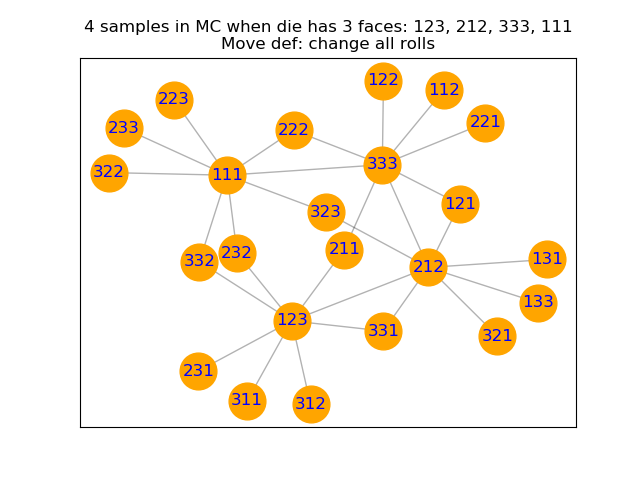
\includegraphics[scale=0.9]{mc_plot}}
	  \caption{All neighboors for states 123, 212, 333, and 111 are shown with Kernel defined as: change all rolls (or entries).}
\end{figure}


\subsection{Running the provided code}
In the graph above, only the states 111, 123, 212, and 333 and all states that communicate with them are shown to avoid a crowded plot.

In this project, we provide a \textbf{code} that simulates a Markov chain with the kernel we just defined. You can run the code by running the setup and then running from the source folder: \textbf{"python3 dependent\_bootstrap n"}, where n is the size of E (number of singletons in the sigma-algebra or number of "entries" in our standard notation if you prefer). Your samples will be saved in the \textbf{"deliverables"} folder, which will be created when you run it for the first time. The program will prevent you from running the code with $n < 3$.


\subsection{Next steps}
Our next steps will be checking that we obtain the desired invariant measures $\pi$ in concrete examples, such as the ones we just saw in the previous sections, and then finally we can compare the asymptotic variance associated to different kernels. If our predications are right, we expect to see lower asymptotic variance when we use kernels that do not allow self re-sampling compared to those that do or the traditional bootstrapping.






